%
% Questa parte spiega un po' l'analogia fra reazioni di doppio scambio di carica e doppio decadimento beta senza neutrini. L'avevo scritta ma cappuzzello mi ha detto di toglierla.
%
Il principale meccanismo di reazione del DCE dipende dal termine isovettoriale dell'interazione nucleone-nucleone; in particolare, nella rappresentazione dell'isospin, le reazioni di DCE sondano le doppie eccitazioni isovettoriali generate dalla combinazione $\tau_{a\pm}\tau_{a\pm}\tau_{A\mp}\tau_{A\mp}$ degli operatori di creazione e annichilazione dell'isospin, la quale agisce rispettivamente su due nucleoni del proiettile e due del bersaglio.
Dunque, analogamente alle reazioni di SCE, i processi di DCE possono essere utilizzati per studiare la risposta nucleare al grado di libertà dell'isospin, sebbene in questo caso si selezionino effetti del secondo ordine.


Il meccanismo di DCE è convenzionalmente descritto come un processo a due step\cite{satchler:87}, caratterizzato dalla successione di due eventi indipendenti di SCE, in cui, dopo il primo evento, il sistema si propaga prima che si verifichi il secondo.
%La descrizione più convenzionale del meccanismo di DCE prevede che esso sia un processo a due step\cite{satchler:87}, caratterizzato dalla successione di due eventi indipendenti di SCE, in cui, dopo il primo evento, il sistema si propaga prima che si verifichi il secondo. 
Dal momento che non c'è alcuna correlazione tra i due eventi di SCE, in questo contesto il DCE si configura come un Double Single Charge Exchange (DSCE). Una rappresentazione grafica del meccanismo è riportata in Figura~\ref{fig:DSCE}.
\begin{figure} [!t]
	\centering
	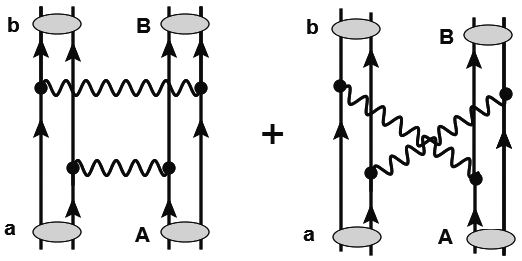
\includegraphics[scale=0.65]{Grafici/DSCE.png}
	\caption{Rappresentazione diagrammatica del meccanismo di Double Single Charge Exchange. La reazione procede attraverso due successivi, ma indipendenti, scambi di mesoni carichi. Figura tratta da \cite{cappuzzello:epja18}.} \label{fig:DSCE}
\end{figure}
%Poiché ciascuno dei processi di SCE è indotto dall'azione di operatori a un corpo sul proiettile e sul bersaglio, tale meccanismo può essere considerato una reazione di DCE a un corpo che avviene in due step. 
Questa descrizione mostra molte analogie con il $2 \nu \beta \beta $, così che sarebbe possibile estrarre informazioni sugli elementi di matrice nucleare di tale decadimento studiando le reazioni di DCE e facendo un confronto con i dati relativi al $2 \nu \beta \beta $.

Nel quadro teorico esiste un meccanismo di reazione di DCE alternativo a quello convenzionale, che manifesta una stretta somiglianza con il \doppiobeta. Secondo tale descrizione, una coppia di nucleoni, correlata attraverso lo scambio di un mesone neutro, cambia la sua carica totale di due unità emettendo una coppia di mesoni carichi. Se il nucleo è isolato, i due mesoni emessi vengono riassorbiti, in modo tale che la carica nucleonica è ristabilita e non c'è un effetto netto. Se, invece, la coppia di mesoni carichi viene assorbita da un secondo nucleo, allora in entrambi i nuclei la carica cambia di due unità, in modo complementare per i due corpi.
Questo meccanismo, chiamato \emph{Majorana-DCE}, a differenza del DSCE avviene in un solo step, come si può notare dal diagramma in Figura~\ref{fig:Majorana-DCE}.
L'aspetto che più di ogni altro distingue le due descrizioni è la correlazione fra i due mesoni. Dal momento che nel \doppiobeta{} esiste una correlazione simile, il Majorana-DCE puàìò essere pensato come la controparte adronica del \doppiobeta.
\begin{figure} [htb]
	\centering
	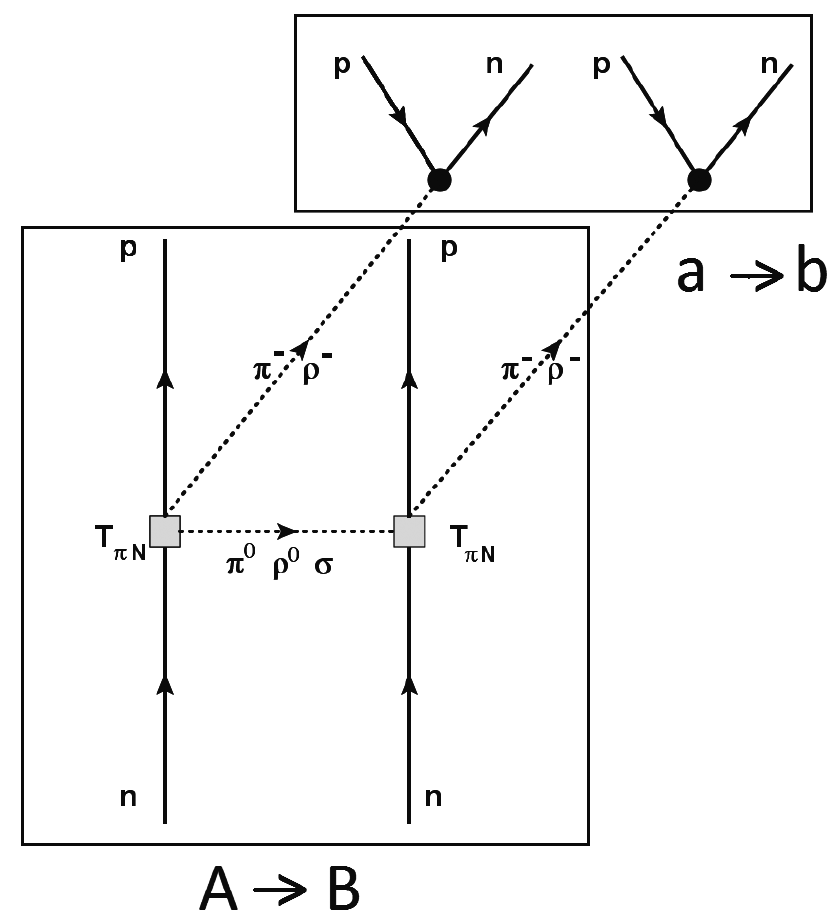
\includegraphics[scale=0.3]{Grafici/Majorana-DCE.png}
	\caption{Rappresentazione diagrammatica del Majorana-DCE per la transizione $n\, n \rightarrow p\,p$. Un processo di scattering virtuale $n\, n \rightarrow p\,p \: \pi^- \,\pi^-$ cambia la carica di due unità nel bersaglio, che passa da $A$ a $B$. Contemporaneamente due protoni nel proiettile assorbono i mesoni carichi, trasformandosi in neutroni. Figura tratta da \cite{cappuzzello:epja18}.} \label{fig:Majorana-DCE}
\end{figure}